\begin{figure*}[t]
\centering
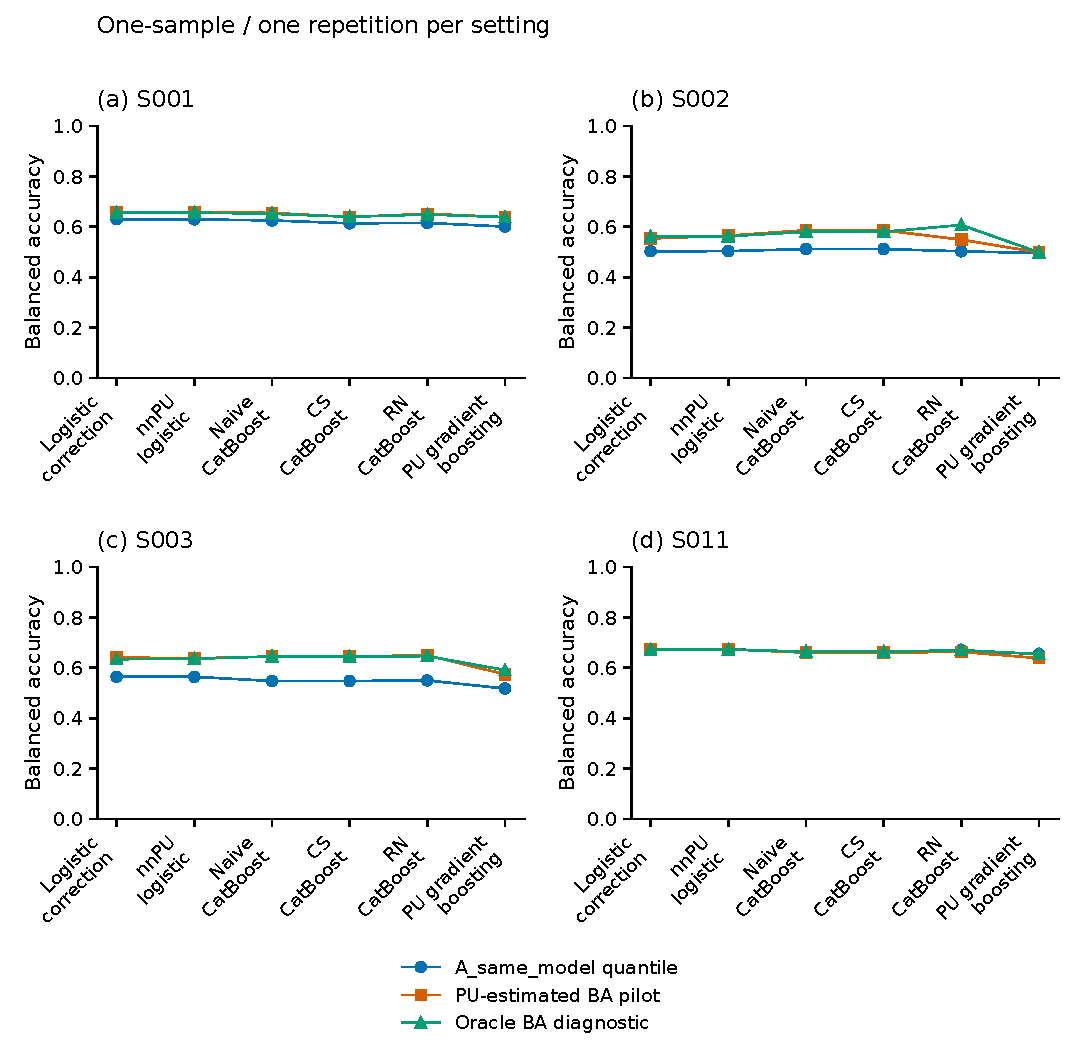
\includegraphics[page=1,width=\textwidth]{mlj_revision/display_package/supplement/figures/fig_s_threshold_sensitivity.pdf}
\caption{Threshold pilot only: eight simulation settings x one repetition per design, plus eight real datasets x two label budgets x one split per design in the table. All three rules apply to the same selected train-only model. A\_same\_model uses the population-representative validation quantile (all validation observations for one-sample; validation U only for two-sample). PU-estimated BA is Task 1C's pilot rule; oracle BA uses true validation labels and is diagnostic only. Test labels never select thresholds. No historical mixed or refit-transfer rule is presented. The figure shows the six conceptual representatives on simulation cases; the table retains all 25 methods and real pilot cases. Six real-data method/case replays failed validation verification and are marked unavailable, leaving 1,194 verified method/case results per rule. One-sample / simulation pilot 1--4. }
\label{fig:fig-s-threshold-sensitivity-page1}
\end{figure*}

\begin{figure*}[t]
\centering
\includegraphics[page=2,width=\textwidth]{mlj_revision/display_package/supplement/figures/fig_s_threshold_sensitivity.pdf}
\caption{Threshold pilot only: eight simulation settings x one repetition per design, plus eight real datasets x two label budgets x one split per design in the table. All three rules apply to the same selected train-only model. A\_same\_model uses the population-representative validation quantile (all validation observations for one-sample; validation U only for two-sample). PU-estimated BA is Task 1C's pilot rule; oracle BA uses true validation labels and is diagnostic only. Test labels never select thresholds. No historical mixed or refit-transfer rule is presented. The figure shows the six conceptual representatives on simulation cases; the table retains all 25 methods and real pilot cases. Six real-data method/case replays failed validation verification and are marked unavailable, leaving 1,194 verified method/case results per rule. One-sample / simulation pilot 5--8. }
\label{fig:fig-s-threshold-sensitivity-page2}
\end{figure*}

\begin{figure*}[t]
\centering
\includegraphics[page=3,width=\textwidth]{mlj_revision/display_package/supplement/figures/fig_s_threshold_sensitivity.pdf}
\caption{Threshold pilot only: eight simulation settings x one repetition per design, plus eight real datasets x two label budgets x one split per design in the table. All three rules apply to the same selected train-only model. A\_same\_model uses the population-representative validation quantile (all validation observations for one-sample; validation U only for two-sample). PU-estimated BA is Task 1C's pilot rule; oracle BA uses true validation labels and is diagnostic only. Test labels never select thresholds. No historical mixed or refit-transfer rule is presented. The figure shows the six conceptual representatives on simulation cases; the table retains all 25 methods and real pilot cases. Six real-data method/case replays failed validation verification and are marked unavailable, leaving 1,194 verified method/case results per rule. Two-sample / simulation pilot 1--4. }
\label{fig:fig-s-threshold-sensitivity-page3}
\end{figure*}

\begin{figure*}[t]
\centering
\includegraphics[page=4,width=\textwidth]{mlj_revision/display_package/supplement/figures/fig_s_threshold_sensitivity.pdf}
\caption{Threshold pilot only: eight simulation settings x one repetition per design, plus eight real datasets x two label budgets x one split per design in the table. All three rules apply to the same selected train-only model. A\_same\_model uses the population-representative validation quantile (all validation observations for one-sample; validation U only for two-sample). PU-estimated BA is Task 1C's pilot rule; oracle BA uses true validation labels and is diagnostic only. Test labels never select thresholds. No historical mixed or refit-transfer rule is presented. The figure shows the six conceptual representatives on simulation cases; the table retains all 25 methods and real pilot cases. Six real-data method/case replays failed validation verification and are marked unavailable, leaving 1,194 verified method/case results per rule. Two-sample / simulation pilot 5--8. }
\label{fig:fig-s-threshold-sensitivity-page4}
\end{figure*}
